\documentclass[20pt,,margin=1in,innermargin=-4.5in,blockverticalspace=-0.25in]{tikzposter}
\geometry{paperwidth=42in,paperheight=32.5in}
\usepackage[utf8]{inputenc}
\usepackage{amsmath}
\usepackage{amsfonts}
\usepackage{amsthm}
\usepackage{amssymb}
\usepackage{mathrsfs}
\usepackage{graphicx}
\usepackage{adjustbox}
\usepackage{enumitem}
\usepackage[backend=biber,style=numeric]{biblatex}
\usepackage{SUtheme}
\usepackage{mathtools}
\usepackage{bm}
\usepackage{bbm}
\setlength{\parindent}{1em}

\usepackage{mwe} % for placeholder images

\addbibresource{refs.bib}

% set theme parameters
\tikzposterlatexaffectionproofoff
\usetheme{SUTheme}
\usecolorstyle{SUStyle}
\usetitlestyle{Filled}

\usepackage[scaled]{helvet}
\renewcommand\familydefault{\sfdefault} 
\usepackage[T1]{fontenc}

% figure support
\usepackage{import}
\usepackage{xifthen}
\usepackage{pdfpages}
\usepackage{transparent}
\newcommand{\incfig}[1]{%
	\def\svgwidth{0.37\columnwidth}
	\import{./Figures/}{#1.pdf_tex}
}

\title{Using Graph Neural Network to Solve the Traveling Salesman Problem}
\author{Pingbang Hu, Jonathan Moore, Yi Zhou, Shubham Kumar Pandey, Anuraag Ramesh}
\institute{University of Michigan}
\titlegraphic{
\includegraphics[width=0.06\textwidth]{Figures/U-M_Logo-Hex.png}}

% begin document
\begin{document}
\maketitle
\centering
\begin{columns}
	\column{0.3}
	\block{Abstract}{
		\par Graph neural network is a rising concept in computer science that has demonstrated significant potential in many areas. Our project aims to
		further explore this potential by applying it to the classic traveling salesman problem. After generating the dataset, we first use imitation
		learning to obtain a pretty good path, which then will be inputted into reinforcement learning to obtain the optimal solution. Since imitation
		learning converges relatively rapidly, the method could be extremely fast compared to traditional exact solvers. Our next steps would be tuning
		the reinforcement learning, and running on larger TSP problems.
	}

	%\block{Motivation}{

	%}

	\block{The Basics of GNN}{
		\par A graph neural network (GNN) is a class of neural network for processing data best represented by graph data structures. They were popularized
		by their use in supervised learning on properties of various molecules.

		\par Since their inception, variants of the message passing neural network (MPNN) framework have been proposed. These models optimize GNNs for use
		on larger graphs and apply them to domains such as social networks, citation networks, and online communities. GNNs have also been relatively
		successful in various NP-hard combinatorial problems, automated planning and path-planning areas due to the inherent graph structure of data.

		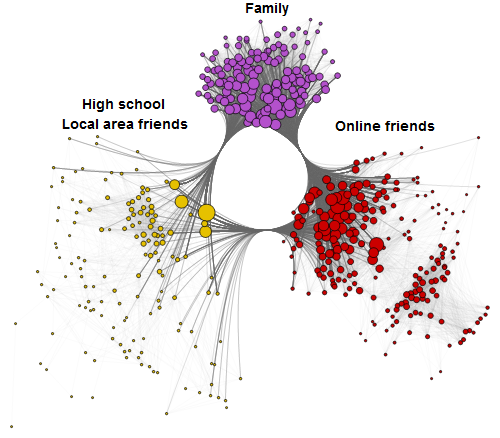
\includegraphics[width=15cm]{Figures/GNN_APP.png}
		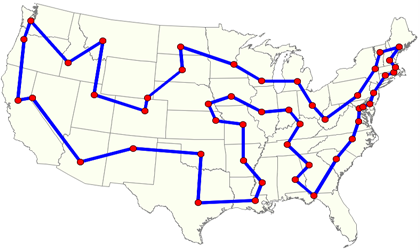
\includegraphics[width=15cm]{Figures/TSP.png}
	}

	% NEW COLUMN
	%\column{0.36}
	\block{Pipeline}{
		%\vspace{1em}
		%\begin{tikzfigure}[Big fancy graphic.]
		%    \includegraphics[width=0.9\linewidth]{example-image}
		%\end{tikzfigure}
		%\vspace{1em}
		%\section{Proposed Method}
		\section{Problem Formulation}
		\subsection{TSP as Integer Linear Programming}
		We first formulate TSP in terms of \textbf{Integer Linear Programming}. Given an undirected weighted group \(\mathcal{G} = (\mathcal{E}, \mathcal{V})\), we label the
		nodes with numbers \(1, \ldots, n\) and define
		\[
			x_{ij}\coloneqq \begin{dcases}
				1, & \text{if }(i, j)\in \mathcal{E}^\prime                       \\
				0, & \text{if } (i, j)\in \mathcal{E}\setminus\mathcal{E}^\prime,
			\end{dcases}
		\]
		where \(\mathcal{E}^\prime\subset \mathcal{E}\) is a variable which can be viewed as a compact representation of all variables \(x_{ij}\), \(\forall i, j\).
		Furthermore, we denote the weight on edge \((i, j)\) by \(c_{ij}\), then for a particular TSP problem instance, we can formulate the problem as follows.
	}
	% NEW COLUMN
	\column{0.4}
	\block{Pipeline (cont.)}{
	We can also divide the original relaxed LP into two sub-problems by \textbf{splitting the feasible region} according to a variable that does not respect
	integrality in the current relaxed LP solution \(\bm{x}^\ast\),
	\begin{equation}\label{eq:branch-and-bound}
		x_{i} \leq \left\lfloor x_{i}^\ast \right\rfloor\lor x_{i} \geq \left\lceil x_{i}^\ast \right\rceil,\qquad \exists i\leq p\mid x_{i} ^\ast \notin \mathbb{\MakeUppercase{z}}.
	\end{equation}

	We see that by adding such additional constraint in two sub-problems respectively, we get a recursive algorithm called \textbf{Branch and Bound}\cite{B&B.ch7}.


	\section{Learning Pipeline}

	Our learning pipeline is as follows. Firstly, we only use imitation learning following \cite{GasseCFCL19} to obtain a good enough model, then we turn to
	unsupervised learning setup under the framework of reinforcement learning, which aims make the network learn some domain-specific property and help to
	boost the performance. The implementation summary can be found in

	\begin{tikzfigure}
		\centering
		\incfig{pipeline}
	\end{tikzfigure}

	\subsection{Imitation Learning}
	As mentioned before, the most effective branching strategy is strong branching, hence we train the network by behavioral cloning
	\cite{Efficient-Training-of-Artificial-Neural-Networks}.\\

	% For line break reasons, above citation shortened from:
	% Efficient-Training-of-Artificial-Neural-Networks-for-Autonomous-Navigation
	We first run the SOTA solver and get state-action pairs:
	\[
		\mathcal{\MakeUppercase{d}} = \left\{(s_{i} , \bm{a} _{i} ^\ast)\right\}_{i = 1}^N,
	\]
	and then learn our policy \(\widetilde{\pi} ^\ast\) b minimizing the cross-entropy loss:
	\[
		\mathcal{\MakeUppercase{l}} (\theta ) = - \frac{1}{N}\sum\limits_{(\bm{s}, \bm{a}^\ast)\in \mathcal{\MakeUppercase{d}} }\log \widetilde{\pi}_\theta (\bm{a} ^\ast \mid \bm{s} ).
	\]

	Additionally, we access (observe) the state of the branch-and-bound process by directly interacting with the SOTA solvers, specifically,
	\texttt{SCIP}. The implementation detail follows Gasse et al.\cite{GasseCFCL19}.
	}
	% NEW COLUMN
	\column{0.3}

	% NEW COLUMN
	%\column{0.32}
	\block{Experimental Results}{
		[TODO]

		% \begin{tikzfigure}[Look, my method is better.]
		%     \includegraphics[width=15cm]{example-image}
		% \end{tikzfigure}
	}

	\block{Conclusion}{
		(Need to discuss together.)
		Even with a fairly limited scope and size of our neural network, we have already
	}

	\block{Future Work}{
		We will implement unsupervised reinforcement learning. After getting a stable model from imitation learning, we remove the expert's
		instructions and let the model explore by itself. Another way to further explore this topic is to perform on larger TSP datasets (e.g. TSP 50).
	}

	\block{References}{
		%TODO
	}

	%\block{References}{
	%    \vspace{-1em}
	%    \begin{footnotesize}
	%    \printbibliography[heading=none]
	%    \end{footnotesize}
	%}
\end{columns}
\end{document}
